در این بخش در ابتدا جهت تست مدل ارائه شده، کد مربوط به مدل پایه را با مقادیر ثابت \مل{12 v} و \مل{6v} برای ولتاژ موتور ها تست نمودیم که نتیجه ان در شکل \رجوع{تست۱} آورده شده است.
\begin{figure}[h]
	\centering
	\includegraphics[width=15cm]{img/test1.jpg}
	\شرح{نتیجه تست بخش مدل ربات}
	\برچسب{تست۱}
\end{figure}
همان طور که انتظار می روود با اعمال مقادیر مختلف ولتاژ به موتورهای ربات، ربات شروع به چرخیدن خواهد نمود که نتایج نیز به درستی این موضوع را نشان می‌دهند.\\
در ادامه شبیه سازی کامل با استفاده از روش تطبیقی و مقادیر بیان شده در مقاله صورت گرفت که نتایج آن در شکل \رجوع{نتایج۱} و شکل \رجوع{نتایج۲} آورده شده است. البته لازم به ذکر می‌باشد که مقادیر اولیه کنترلر که در مقاله ذکر نشده بود، برابر ۰ در نظر گرفته شد. \\
\begin{figure}[h]
	\begin{center}
		\subfigure[]{
			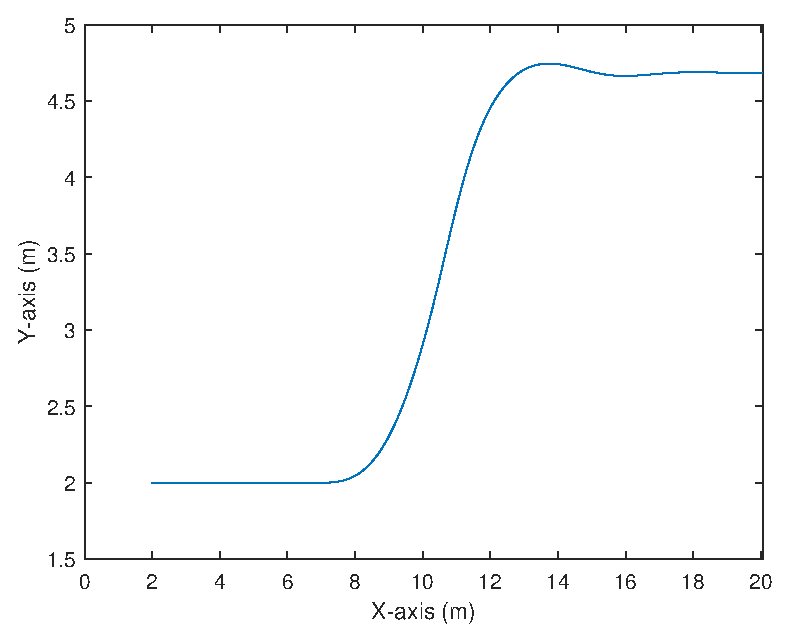
\includegraphics[height=7cm,width=7cm]{img/fig-2A-xy}  
			\label{2A-xy}
		}
		\hspace*{0.2cm}
		\subfigure[]{
			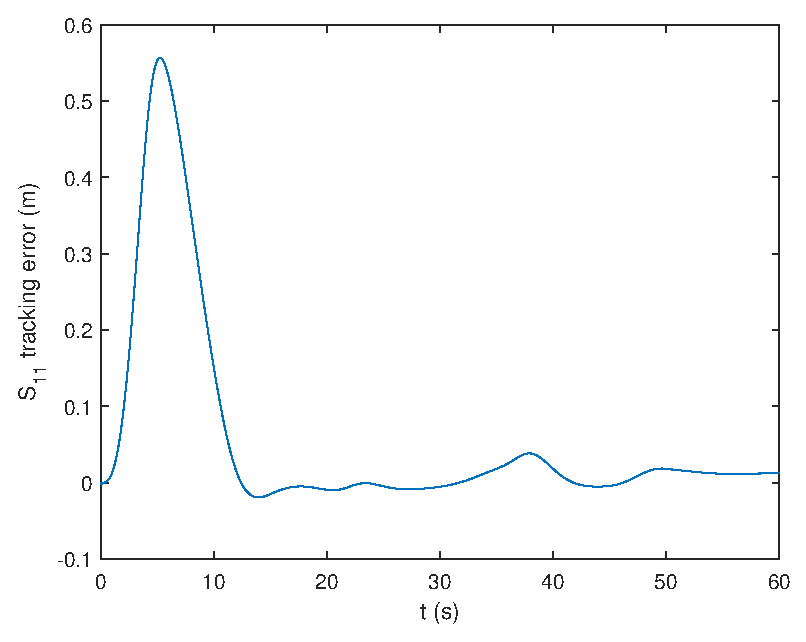
\includegraphics[height=7cm,width=7cm]{img/fig-2B-s11} 
			\label{2B-s11}
		}
	\subfigure[]{
		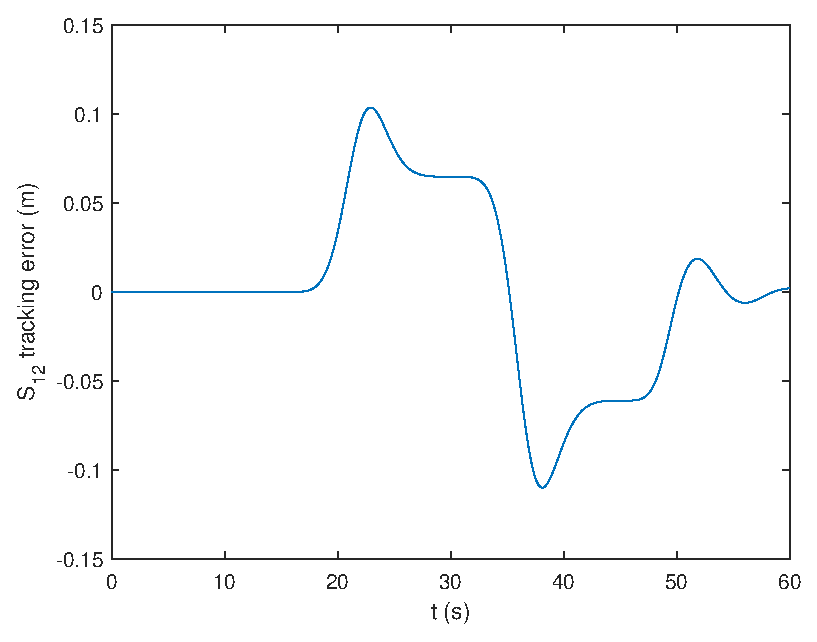
\includegraphics[height=7cm,width=7cm]{img/fig-2C-s12}  
		\label{2C-s12}
	}
	\hspace*{0.2cm}
	\subfigure[]{
		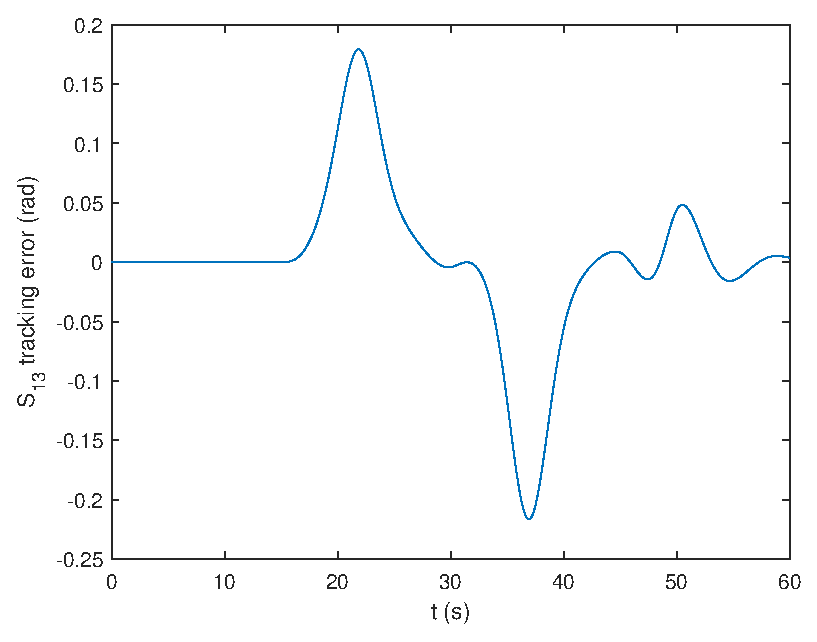
\includegraphics[height=7cm,width=7cm]{img/fig-2D-s13}  
		\label{2D-s13}
	}
	\end{center}
	\caption{
		\subref{2A-xy} نتیجه ردیابی مسیر
		\subref{2B-s11} خطای ردیابی \مل{$s_{11}$}
		\subref{2C-s12} خطای ردیابی \مل{$s_{12}$} 
		\subref{2D-s13} خطای ردیابی \مل{${\bar{s}}_{13}$} 
	}
\برچسب{نتایج۱}
\end{figure}
\begin{figure}[h]
	\begin{center}
		\subfigure[]{
			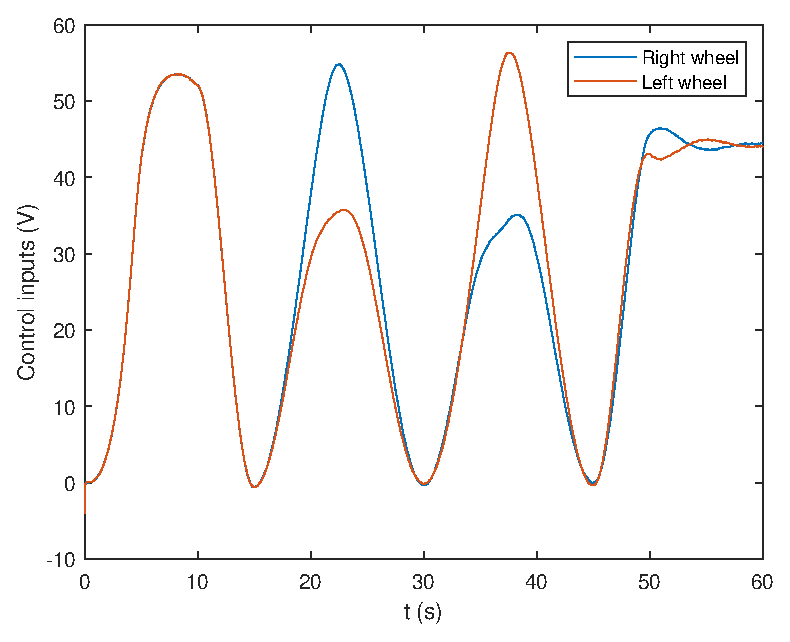
\includegraphics[height=7cm,width=7cm]{img/fig-3A-v}  
			\label{3A-v}
		}
		\hspace*{0.2cm}
		\subfigure[]{
			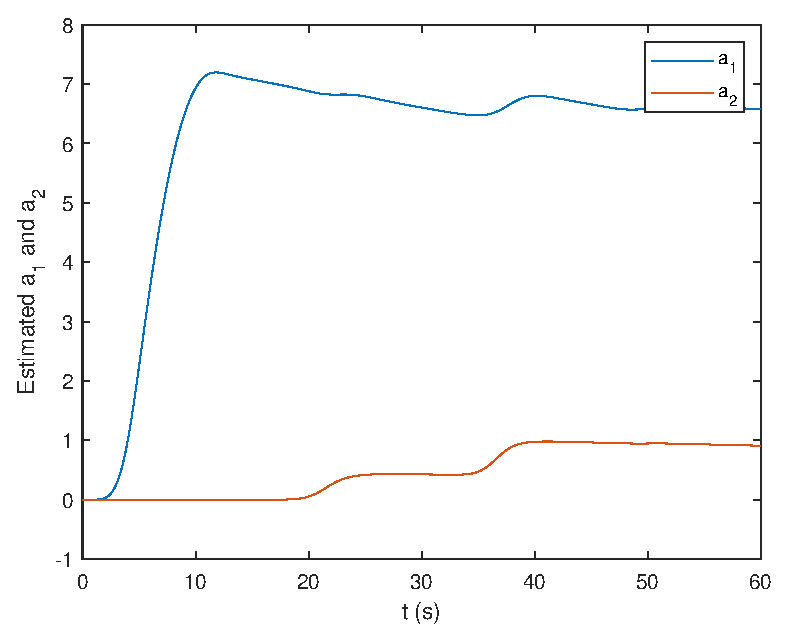
\includegraphics[height=7cm,width=7cm]{img/fig-3B-a1-a2} 
			\label{3B-a1-a2}
		}
		\subfigure[]{
			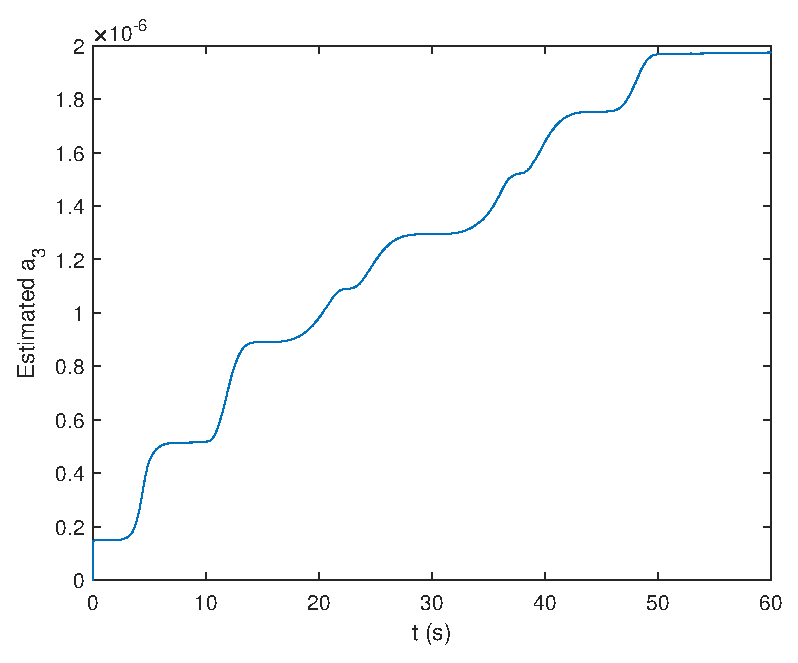
\includegraphics[height=7cm,width=7cm]{img/fig-3C-a3}  
			\label{3C-a3}
		}
		\hspace*{0.2cm}
		\subfigure[]{
			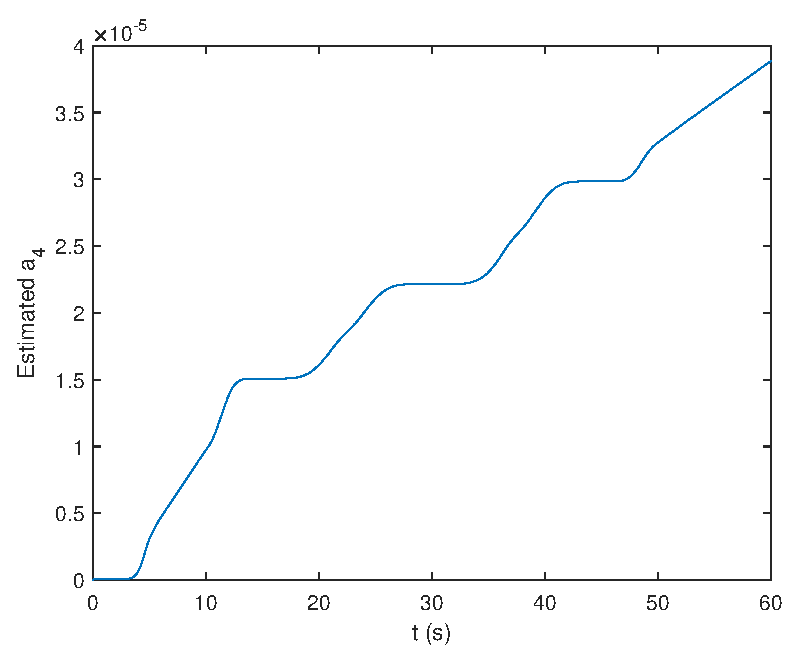
\includegraphics[height=7cm,width=7cm]{img/fig-3D-a4}  
			\label{3D-a4}
		}
	\end{center}
	\caption{
		نتایج حاصل از شبیه سازی
		\subref{3A-v} ورودی کنترلی
		\subref{3B-a1-a2} پارامتر تخمین زده شده
		\subref{3C-a3} پارامتر تخمین زده شده
		\subref{3D-a4} پارامتر تخمین زده شده
	}
\برچسب{نتایج۲}
\end{figure}
\begin{figure}[h]
	\centering
	\includegraphics[height=15cm,width=15cm]{img/article_result1}
	\شرح{نمودار های معادل شکل \رجوع{نتایج۱} در مقاله \آ}
	\برچسب{نتایج-مقاله-۱}
\end{figure}
\begin{figure}[h]
	\centering
	\includegraphics[height=15cm,width=15cm]{img/article_result2}
	\شرح{نمودار های معادل شکل \رجوع{نتایج۲} در مقاله \آ}
	\برچسب{نتایج-مقاله-۲}
\end{figure}
از مقایسه نمودار های رسم شده در مقاله (شکل \رجوع{نتایج-مقاله-۱}،
 شکل \رجوع{نتایج-مقاله-۲}) و نتایج حاصل از شبیه سازی مشاهده می‌شود نتایج شبیه سازی در بسیاری از موارد با نتایج مقاله هم خوانی دارد. البته در برخی از نمودار ها تفاوت های جزئی مشاهده می‌شود که دلایل آن را می‌توان به طور خلاصه این طور بیان کرد:
\شروع{فقرات}
\فقره از آنجاییکه شرایط اولیه کنترلر در مقاله ذکر نشده است ممکن است مقادیر در نظر گرفته شده در مقاله با مقادیر شبیه سازی شده در این تحقیق متفاوت باشد.
\فقره اغتشاش رندوم استفاده شده در شبیه سازی، قابلیت تکرار ندارد. 
\پایان{فقرات}
\begin{figure}[h]
	\centering
	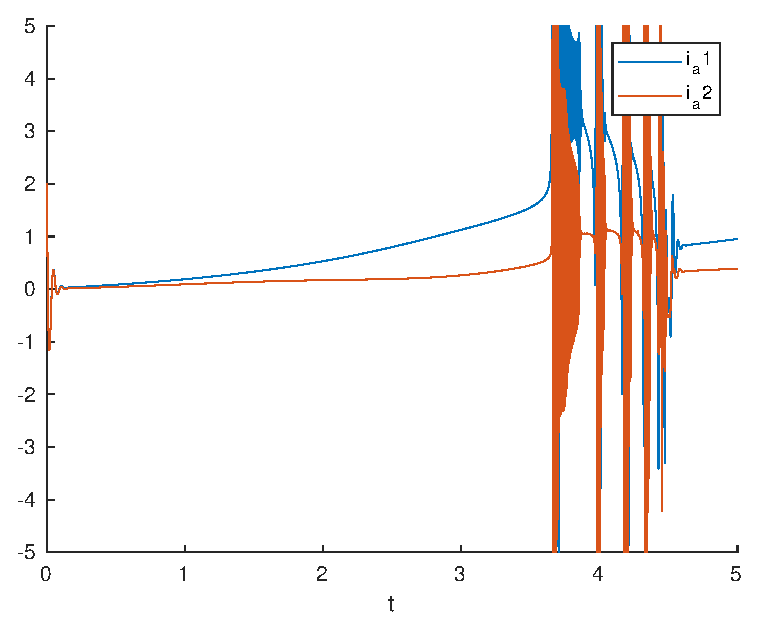
\includegraphics[height=8cm,width=8cm]{img/fig-unstable}
\end{figure}